\subsection{Modulo Principal}

Este módulo está formado por el archivo, \texttt{MAIN\_POWER.ino} que se encarga de conectar todos los módulos en un sistema unificado.

Inicialmente, en la cabecera del fichero se incluyen las librerías que vamos a utilizar:
\begin{itemize}
    \item \texttt{telemetry.hpp}: Define la estrucura de datos que será usarda para almacenar las lecturas recibidas por los INAs.
    \item \texttt{hardware-hpp}: Define los pines del ESP que son necesarias para el funcionamiento del sistema (I2C y relés).
    \item \texttt{ina.hpp}: Contiene el codigo relativo a la gestión, configuración y obtención de datos de los INAs. 
    \item \texttt{mqtt\_client.hpp}: Contiene el codigo relativo a la conexión y envio de datos al servidor MQTT.
    \item \texttt{file\_management.hpp}: Contiene el codigo relativo a la escritura en un fichero de los datos recibidos de los INA.
    \item \texttt{sleep.hpp}: Contiene el codigo que pone en bajo consumo al ESP.
\end{itemize}

\begin{lstlisting}[captionpos=b, caption={Cabecera con los módulos y ficheros utilizados}, language=c++]
    #include "telemetry.hpp"
    #include "hardware.hpp"
    #include "ina.hpp"
    #include "mqtt_client.hpp"
    #include "file_management.hpp"
    #include "sleep.hpp"
\end{lstlisting}

A continuación, se cuenta define un elemento que puede ser usado para debugear el código:
\begin{lstlisting}[captionpos=b, caption={Definición del debuger}, language=c++]
    #define DEBUG

    #ifdef DEBUG
    #define PRINT_DEBUG(...) Serial.println(__VA_ARGS__)
    #else
    #define PRINT_DEBUG(...)
    #endif    
\end{lstlisting}

A lo largo del codigo de este programa se hacen varias llamadas al metodo \texttt{PRINT_DEBUG(...)}, este metodo se encarga de escribir por el puerto serie información de interes como:
\begin{itemize}
    \item Mostrar la información recibida por los INAs (asi corroborar la correcta recepción en el MQTT).
    \item Indicar si se ha podido enviar correctamente los datos al servidor MQTT.
    \item Indicar la hora recibida del NTP.
    \item Indicar la correcta conexión con la red Wifi.
    \item Indicar si se ha podido escribir correctamente en el fichero que almacena los datos de medidas.
    \item Indicar el estado del proceso de conexión con la WIFI.
    \item Indicar las modificaciones en los relés y el estado en el que se encuentran.
\end{itemize}

Después de este código, se encuentra la definición de distintos elementos utilizados por el main:
\begin{lstlisting}[captionpos=b, caption={DEFINES de MAIN_POWER}, language=c++]
    #define ssid             "POC"
    #define password         "POWERIoT"
    
    #define MQTT_SERVER      const_cast<char*>("192.168.111.69")
    #define MQTT_PORT        4444
    
    #define TIME_SLEEP       2000
    #define WIFI_TRIES       35
    #define BAT_THRESH       11.65
    #define SOLAR_THRESH     20
    #define MEASUREMENT_FILE "/measurements.txt"
\end{lstlisting}

\begin{itemize}
    \item \texttt{ssid y password}: Son utilizados para indicar el ssid de la wifi a la que conectarse y su contraseña. 
    \item \texttt{MQTT_SERVER y MQTT_PORT}: Indican la dirección y el puerto del servidor MQTT al que el ESP se intentará conectar para enviar datos.
    \item \texttt{TIME_SLEEP}: Indica el tiempo en ms que se quedará en bajo consumo/dormido el sistema.
    \item \texttt{WIFI_TIRES}: Indica el numero de reintentos que damos al ESP para conectarse a la red wifi.
    \item \texttt{BAT_THRESH}: Umbral de la batería de backup con el que el sistema determina si activa la protección de sobrecarga.
    \item \texttt{SOLAR_THRESH}: Umbral del panel solar para el que el sistema determina si cambiamos a la carga mediante la batería de backup.
    \item \texttt{MEASUREMENT\_FILE}: Indica la ruta donde se almacena el fichero de medidas.
\end{itemize}

El fichero contiene las siguientes funciones:

- \texttt{setup()}: Inicializa los pines que usamos para la comunicación I2C y los relés, la velocidad del puerto serie y el valor inicial de la estructura de datos que contienen.

\begin{lstlisting}[captionpos=b, caption={Codigo de la funcion setup}, language=c++]
    void setup() {
        pinMode(RELAY_SW_IN,  OUTPUT);
        pinMode(RELAY_SW_OUT, OUTPUT);
        pinMode(SDA,          OUTPUT);
        pinMode(SCL,          OUTPUT);
    
        Serial.begin(9600);
    }    
\end{lstlisting}

- \texttt{loop()}: Realiza todas las operaciones de funcionamiento del sistema. La secuencia de ejecución es la siguiente:
\begin{enumerate}
    \item Recoge las medidas de los INA.
    \item Revisa los valores obtenidos del panel solar por si es necesario cambiar la alimentación del panel solar a la de backup.
    \item Se intenta conectar a la red Wifi. Si lo consigue se intenta mandar las medidas al servidor mqtt.
    \item Guarda las medidas de los sensores en un fichero.
    \item Duerme al ESP poniéndolo en bajo consumo.
    \item Sale del modo de bajo consumo.
\end{enumerate}

\begin{lstlisting}[captionpos=b, caption={Codigo de la funcion loop}, language=c++]
    measureINA226(&telemetry); // Si no están los INA conectados, bloquea

    PRINT_DEBUG("[INA] VSolar [V]:  " + String(telemetry.VSolar));
    PRINT_DEBUG("[INA] ISolar [mA]: " + String(telemetry.ISolar));
    PRINT_DEBUG("[INA] VBatbu [V]:  " + String(telemetry.VBatbu));
    PRINT_DEBUG("[INA] IBatbu [mA]: " + String(telemetry.IBatbu));
    PRINT_DEBUG("[INA] VBat1 [V]:   " + String(telemetry.VBat1));
    PRINT_DEBUG("[INA] IBat1 [mA]:  " + String(telemetry.IBat1));
    PRINT_DEBUG("[INA] VBat2 [V]:   " + String(telemetry.VBat2));
    PRINT_DEBUG("[INA] IBat2 [mA]:  " + String(telemetry.IBat2));

    setRelays(&telemetry);

    setup_wifi();

    if (WiFi.status() == WL_CONNECTED){
        configTime(3600, 0, "time.nist.gov", "0.pool.ntp.org");
        
        if (!publishTelemetry(MQTT_SERVER, MQTT_PORT, telemetry)){
            PRINT_DEBUG("[POWER] ERROR publicando medidas");
        } else {
            PRINT_DEBUG("[POWER] Medidas publicadas con éxito");
        }

        getLocalTime(&currentTime, 1000);
        strftime(timeStr, 50, "[%d/%m/%y - %H:%M:%S]", &currentTime);
        PRINT_DEBUG("[WIFI] Sincronizado con NTP. Hora obtenida: " + String(timeStr));
    } else {
        PRINT_DEBUG("[WIFI] No se ha podido conectar a la red WiFi");
        snprintf(timeStr, 50, "[00/00/00 - 00:00:00]");
    }

    if (write_meas(MEASUREMENT_FILE, telemetry, timeStr)){
        PRINT_DEBUG("[POWER] Fichero escrito con exito");
    } else {
        PRINT_DEBUG("[POWER] El fichero no ha podido ser escrito");
    }

    sleep_low_power(TIME_SLEEP);
\end{lstlisting}

La primera secuencia que hay en el código es \texttt{measureINA226(&telemetry);} función tiene una ligera limitación, si los INAs no han sido inicializados el sistema se queda bloqueado.
Esto ocurre ya que se queda a la espera de una respuesta de la dirección I2C del INA al que esta llamando, que en caso de no estar configurado, se quedará el sistema bloqueado hasta esa respuesta o un rest.

Tras recibir las medidas, si nos encontramos depurando el código, podremos observar por el puerto serie los datos que han sido almacenados de cada elemento del circuito.

Una vez leidas las medidas, el sistema verifica los valores de tensión del panel solar y de la batería y modifica los relés en funcion de estos.
En caso de que no se supere un valor mínimo de tensión tanto del panel solar como de la batería de buckup, el sistema activaría la protección de sobredescarga para evitar daños en el sistema. 
Entrar en este modo implicaría que las funciones del ESP dejarían de estar disponibles hasta que las tensiones superen los umbrales, alimentando una vez mas al ESP y volviendo a su funcionamiento normal.

Tras esto, se intenta la conexión con la red Wifi:
\begin{itemize}
    \item No se consigue conectar a la Wifi: Se establece la hora y fecha de las medidas realizadas a 0 y no se intenta enviar los datos al servidor MQTT. 
    \item Si se consigue conectar a la Wifi: Se configura un servidor NTP para asegurar la fecha y hora en las que realizan las medidas. Tras esto se intena enviar los datos leidos al servidor MQTT.
\end{itemize}

Independientemente de si se ha podido conectar a la Wifi o no, se intenta realizar una escritura con las lecturas realizadas en el fichero de medidas.

Finalmente, tras realizar todas las operaciones anteriores, se pone a dormir el ESP durante un tiempo \texttt{TIME\_SLEEP}. Tras esto el sistema se vuelve a activar y a realizar las operaciones de nuevo.

\begin{figure}[H]
    \centering
    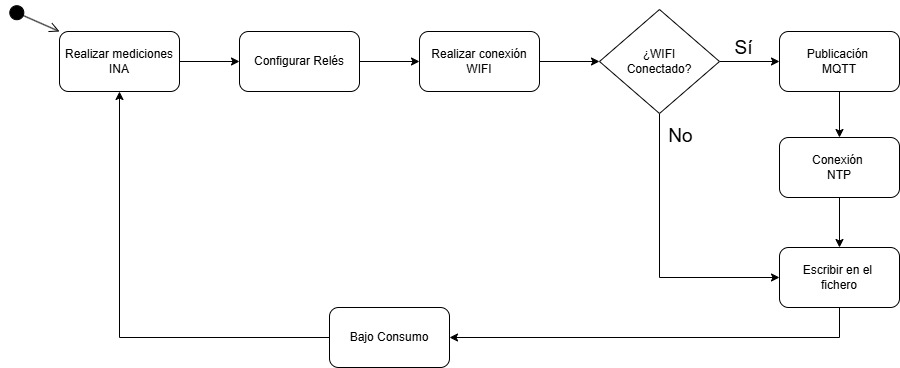
\includegraphics[width=0.95\textwidth]{images/3-software/3-3-programaprincipal/DiagramaDeFlujoPOWER.jpg}
    \caption{Diagrama de flujo Programa Principal}
    \label{fig:3-3-1-DiagramaFlujo}
\end{figure}

Para la implementación del programa principal, también se han desarrollado dos funciones adicionales que se encargan de intentar la conexión WIFI y configurar los relés del sistema. A continuación, se explican dichas funciones:

\begin{itemize}
    \item Función \texttt{setup\_wifi()}: esta función es la encargada de la conexión WIFI del sistema. Se intentará la conexión un número determinado de intentos, definidos en la variable \texttt{WIFI\_TRIES}. Esta función no recibe ningún parámetro y tampoco devuelve nada.
    \begin{lstlisting}[captionpos=b, caption={Definición función setup\_wifi}, language=c++]
        static void setup_wifi();
    \end{lstlisting}
    La secuencia de ejecución de esta función es la siguiente:
    \begin{enumerate}
        \item Muestra por serial un mensaje con la red WIFI a la que se intenta la conexión.
        \item Intenta realizar la conexión a la red WIFI con las credenciales almacenadas en las variables \texttt{ssid} y \texttt{password}. Estas variables almacenan el nombre de la red WIFI y su correspondiente contraseña, respectivamente.
        \item Se intenta realizar la conexión un número finito de intentos indicados en la variable

        \texttt{WIFI\_TRIES}. El tiempo de espera entre intentos de conexión es de 500ms.
        \item En caso de que la conexión haya sido satisfactoria, el sistema mostrará por serial un mensaje al usuario indicando que la conexión WIFI se ha realizado correctamente. En este mensaje se mostrará el nombre de la red a la que se ha realizado la conexión y la dirección IP de nuestro dispositivo ESP8266.
        \item Por otra parte, en caso de que el sistema no haya sido capaz de conectarse a la red WIFI indicada, se mostrará un mensaje de error por serial indicando al usuario la conexión fallida.
    \end{enumerate}
    \begin{lstlisting}[captionpos=b, caption={Desarrollo función setup\_wifi}, language=c++]
        static void setup_wifi() {
            delay(10);
            Serial.print("[WIFI] Intentando conectar a " ssid);
            WiFi.begin(ssid, password);
            for (int i = 0; i < WIFI_TRIES && WiFi.status() != WL_CONNECTED; i++) {
                delay(500);
                Serial.print(".");
                i++;
            }
            if (WiFi.status() == WL_CONNECTED) {
                PRINT_DEBUG("[WIFI] Conectado a la red WiFi " ssid " con IP: ");
                PRINT_DEBUG(WiFi.localIP());
            } else {
                PRINT_DEBUG("[WIFI] No se ha podido conectar a la red WiFi");
            }
        }
    \end{lstlisting}
    \item Función \texttt{setRelays}: esta función es la encargada de configurar los relés del sistema en función de los valores medidos por los sensores y de los valores almacenados en las variables \texttt{SOLAR\_THRESH} y \texttt{BAT\_THRESH}. Esta función recibe como parámetro un puntero a la vabiable \texttt{telemetry}, la cual almacena las medidas obtenidas por los diferentes sensores y no devuelve nada.
    \begin{lstlisting}[captionpos=b, caption={Definición función setRelays}, language=c++]
        static void setRelays(telemetry_t *telemetry);
    \end{lstlisting}
    Esta función se compone de tres casos para las diferentes posibilidades de funcionamiento del sistema. Estas opciones son las siguientes:
    \begin{itemize}
        \item VSolar $>$ \texttt{SOLAR\_THRESH}: esta posibilidad se refleja cuando la tensión medida en el panel solar es mayor al valor del \texttt{threshold} solar, almacenado en dicha variable. Esto quiere decir que la energía aportada por el panel solar es suficiente para asegurar el correcto funcionamiento y cargar de forma adecuada tanto la batería de backup como las otras dos baterías de carga. En este caso, ambos relés están en la posición que hemos denominado \texttt{LOW}, conectando el panel solar y la batería de backup al resto del sistema.
        \item VBatbu $>$ \texttt{BAT\_THRESH}: en caso de que la tensión medida en el panel solar no sea suficiente para alimentar el circuito completo, se comprobará si la energía almacenada en la batería de backup es suficiente. Para ello, se compara la tensión medida en dicha batería con su respectivo \texttt{threshold}, almacenado en la variable \texttt{BAT\_THRESH}. En caso de que dicha tensión medida sea mayor, quiere decir que es suficiente para asegurar el correcto funcionamiento del sistema y la carga correcta de las otra dos batería. Para este caso, los relés conmutan a la posición denominada \texttt{HIGH}, la cual desconecta el panel solar del sistema y conecta la batería de backup al camino de alimentación del sistema.
        \item Por último, en caso de que ni la energía del panel solar ni la de la batería de backup sean suficientes para alimentar el circuito y cargar las dos baterías, se entiende que no hay manera de asegurar el correcto funcionamientod el sistema, por lo que los relés volveran a la posición inicial \texttt{LOW} pero, debido a que no hay alimentación suficiente, el sistema de apagará. El sistema permanecerá en este estado hasta que el panel solar vuelva a su funcionamiento nominal y pueda aportar la cantidad de energía suficiente para volver al comportamiento predeterminado del sistema, cargando tanto la batería de backup como las otras 2 baterías de carga.
    \end{itemize}
    \begin{lstlisting}[captionpos=b, caption={Desarrollo función setRelays}, language=c++]
        static void setRelays(telemetry_t *telemetry){
            if (telemetry->VSolar > SOLAR_THRESH) {
                PRINT_DEBUG("[RELAY] Panel solar activo");

                digitalWrite(RELAY_SW_IN,LOW);
                digitalWrite(RELAY_SW_OUT,LOW);
            } else if (telemetry->VBatbu > BAT_THRESH){
                PRINT_DEBUG("[RELAY] Bateria backup activa");

                digitalWrite(RELAY_SW_IN,HIGH);
                digitalWrite(RELAY_SW_OUT,HIGH);
            } else {
                PRINT_DEBUG("[RELAY] Activando proteccion sobredescarga. Se detendra el sistema");

                digitalWrite(RELAY_SW_IN,LOW);
                digitalWrite(RELAY_SW_OUT,LOW);
            }
        }
    \end{lstlisting}
\end{itemize}
